\section{Joint Model}
\label{sec:joint}

\begin{frame}{Joint Model}{Estimation of Vine Copula}
    \begin{enumerate}
    \item<2-> Transform the standardised residuals from each marginal model with its distribution function, i.e.\ \(t\)- and skew-\(t\)-distributions with estimated shape and skew parameters
    \item<3-> Sequentially fit vine copula, where
      \begin{itemize}
      \item<4-> Edge weights used for MST algorithm are empirical Kendall's \(\tau\)'s
      \item<5-> Each edge is tested for independence
      \item<6-> Pair-copulas considered are: Gaussian, Student's \(t\), Clayton, Gumbel, Frank, and Joe, and their rotations
      \item<7-> Pair-copulas are chosen with BIC
      \end{itemize}
    \item<8-> Reestimate with MLE
    \end{enumerate}
\end{frame}

\begin{frame}{Joint Model}{Summary of Results}
  \begin{center}
    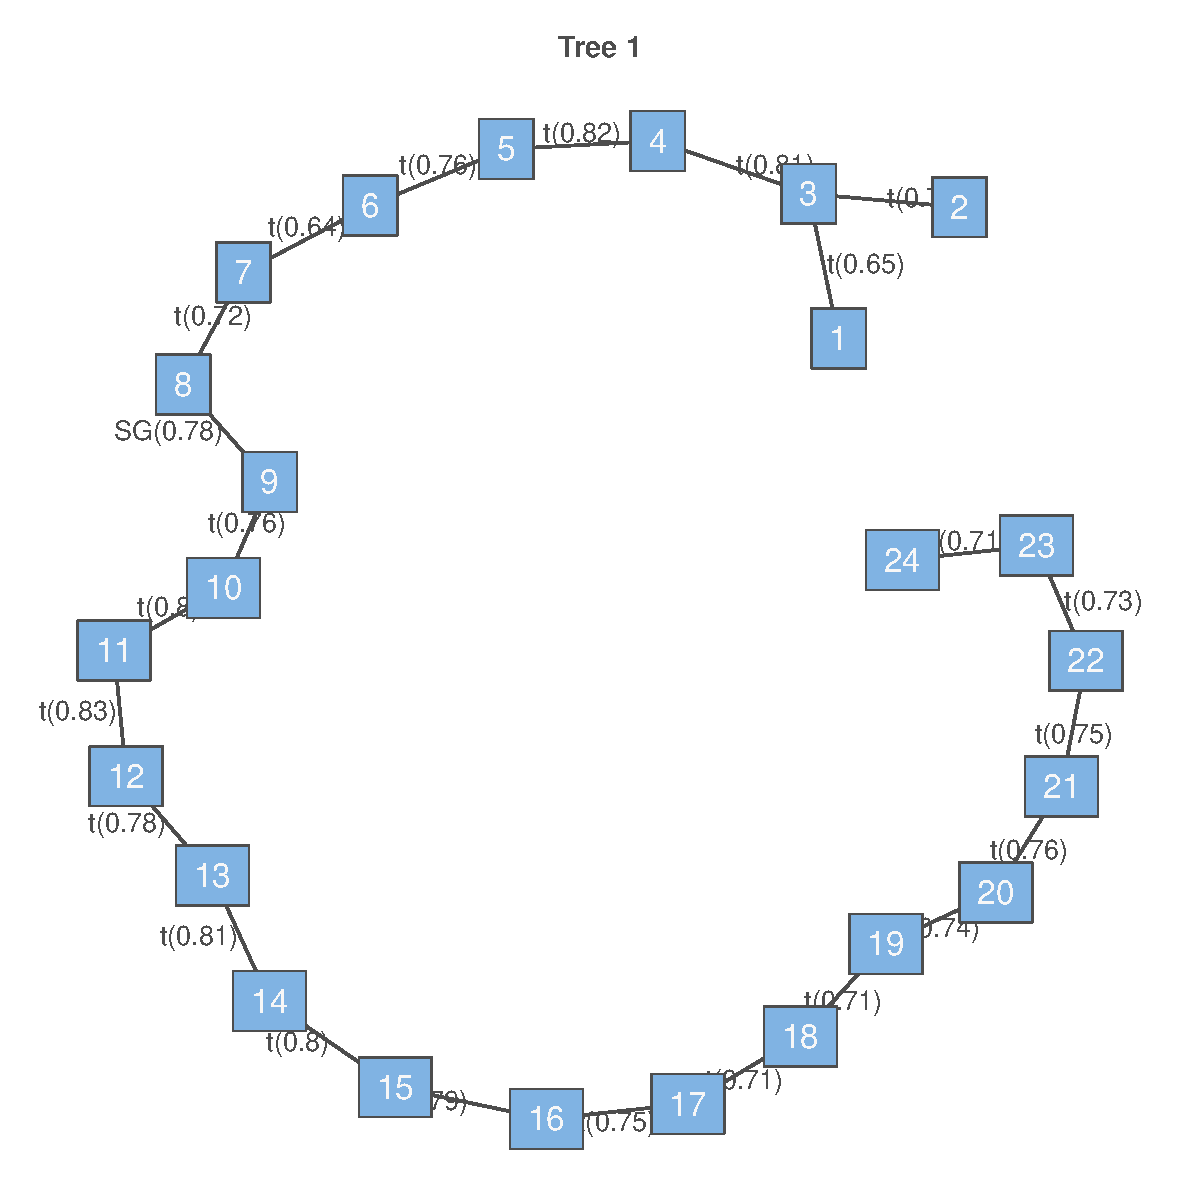
\includegraphics[width=0.6\textwidth]{img/vine}
  \end{center}
\end{frame}

\begin{frame}{Joint Model}{Summary of Results}
  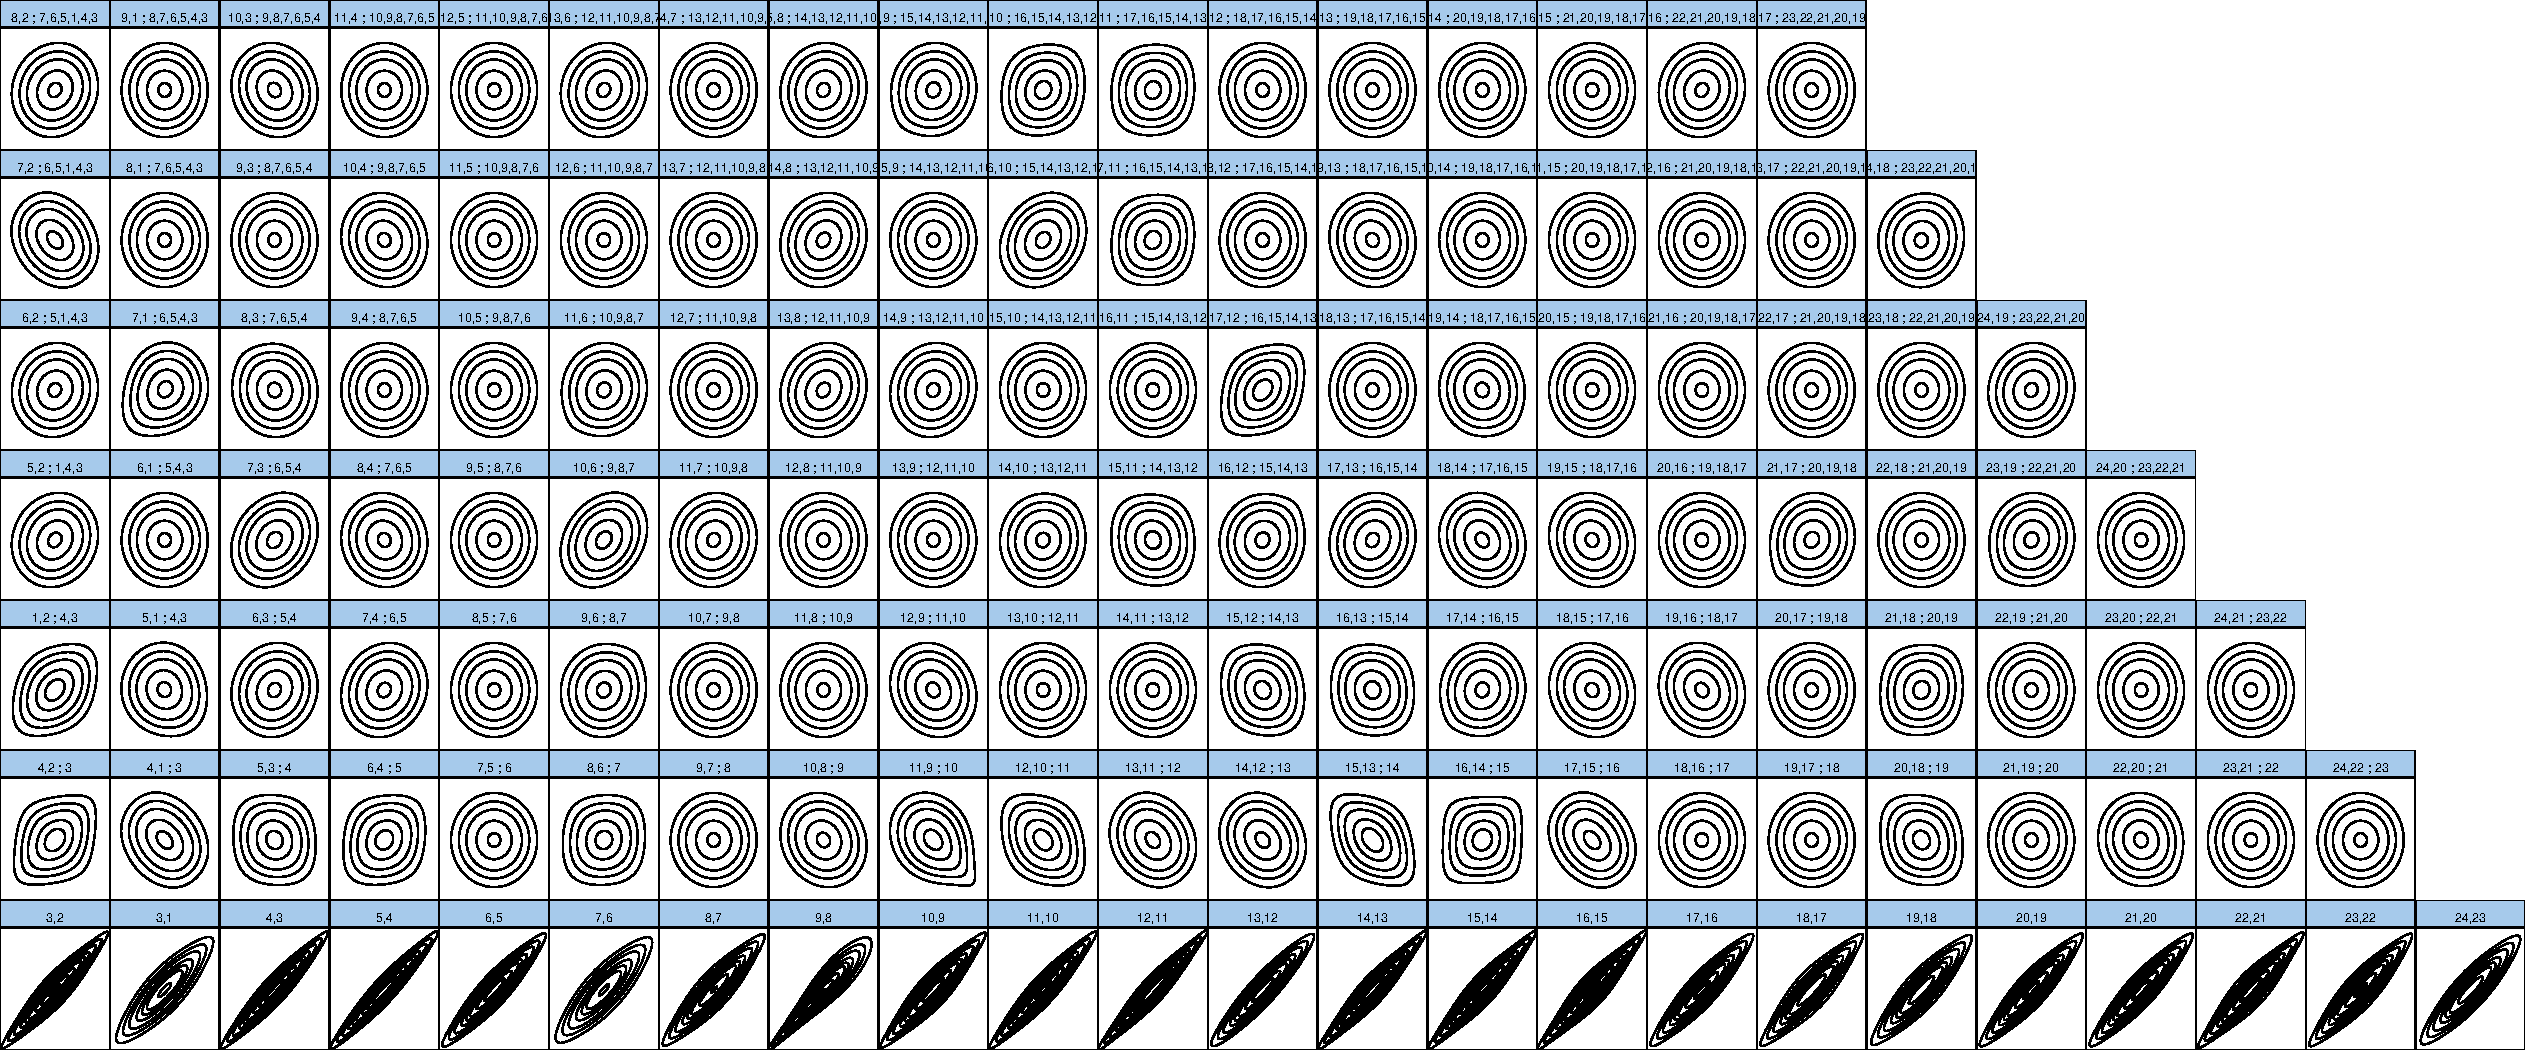
\includegraphics[width=\textwidth]{img/vine-densities}
\end{frame}

\begin{frame}{Joint Model}{Summary of Results}
  \begin{itemize}
  \item<2-> Very close to D-vine structure
  \item<3-> Many (but but not all) \(t\)-copulas in first tree
  \item<4-> Strong, positive dependence in first tree, including tail dependence
  \item<5-> A lot of independence or ``near-independence'' in later trees, in particular tree 19, 21, 22, 23, and 24
    \begin{itemize}
    \item For tree 5 and later, over half of the edges are independence copulas
    \item In total, about 53\% of the copulas are independence copulas
    \item On the other hand, dependence persists until tree 20
    \end{itemize}
  \end{itemize}
\end{frame}

%%% Local Variables:
%%% mode: latex
%%% TeX-master: "../slides"
%%% End:
